\documentclass[12 pt]{article}
\usepackage[english]{babel}
\usepackage{soul}
\usepackage{amsmath}
\usepackage{enumitem}
\usepackage{mathrsfs}
\usepackage{amssymb}
\usepackage{amsthm}
\usepackage{verbatim}
\usepackage{fancyvrb}
%\usepackage{fullpage}
%\usepackage[compact]{titlesec}
\usepackage{listings}
\usepackage[letterpaper, margin=.6 in]{geometry}
\usepackage{times}
\usepackage{setspace}
\singlespacing 
\usepackage{graphicx}%
\usepackage{xfrac}
\usepackage{float}
\usepackage{multicol}
\usepackage{caption}
\usepackage{afterpage}
\usepackage{varwidth}
\usepackage{tikz}

\DeclareGraphicsExtensions{.png}
\graphicspath{{/home/rachellonchar/Dropbox/python_work/peat_project/g/net_inundation_aeration_periods/periods_as_MPPs/}, {/home/rachellonchar/Dropbox/python_work/peat_project/g/net_inundation_aeration_periods/}, {/home/rachellonchar/Dropbox/python_work/peat_project/g/}}

%DOCUMENT HEADER:
\usepackage{fancyhdr}
\pagestyle{fancy}
\lhead{Template Assignment}\usepackage[section]{placeins}
\rhead{Rachel Lonchar}
\cfoot{Page \thepage} %page numbering 
\renewcommand{\headrulewidth}{0.4pt}
\renewcommand{\footrulewidth}{0.4pt}
%

% Declare bold typewriter font with Computer Modern
\DeclareFontShape{OT1}{cmtt}{bx}{n}{<5><6><7><8><9><10><10.95><12><14.4><17.28><20.74><24.88>cmttb10}{}
%\begin{comment}
\usepackage{color}
\definecolor{codegreen}{rgb}{0,0.6,0}
\definecolor{codegray}{rgb}{0.5,0.5,0.5}
\definecolor{codepurple}{rgb}{0.58,0,0.82}
\definecolor{backcolour}{rgb}{0.95,0.95,0.92}
\lstdefinestyle{mystyle}{
    rulecolor=\color{codegray}, 
    basicstyle=\footnotesize\upshape\ttfamily,  
    keywordstyle=\color{blue}\bfseries,
    numberstyle=\tiny\color{codegray},
    commentstyle=\color{codegreen},
    breakatwhitespace=false,         
    breaklines=true,                 
    captionpos=b,                    
    keepspaces=true,  
    frame=single,	                 
    numbers=left,                    
    numbersep=5pt,                  
    showspaces=false,                
    showstringspaces=false,
    stringstyle=\color{codepurple},
    showtabs=false,                  
    tabsize=2}
\lstset{style=mystyle}
%\end{comment}
\newcommand*\lstinputpath[1]{\lstset{inputpath=#1}}
%
%COMMENT OUT
\lstset{inputpath=/home/rachellonchar/Dropbox/python_work/00py_projects/template_category/template_project/code/}

\usetikzlibrary{arrows,positioning} 
\tikzset{
    %Define standard arrow tip
    >=stealth',
    %Define style for boxes
    punkt/.style={
           circle,
           draw=black, thick,
           text width=2em,
           minimum height=2em,
           text centered},
    % Define arrow style
    pil/.style={
           ->,
           thick,
           shorten <=2pt,
           shorten >=2pt,}
}
%
%COMMENT IN 
%\lstset{inputpath=./code}
%----------------------------------------------------------------------------
\begin{document}
\section{Methane emissions as a function of soil temperature and water table}
Methane emissions are well-explained by soil temperature, but deviations from this fit lead us to believe there are other factors at work. Considering methane production is an anaerobic process, it's reasonable to consider the roll of hydrology in methane production. 
%FIG 3
\begin{figure}[!htb]
\centering
\includegraphics[width=.8\textwidth]{Ts10_vs_CH4}
\caption{Methane can be modeled as a exponential function of soil temperature. }
\end{figure}

Goal:
\[CH_4 = f(T_{soil},WT) \]

We can further assume a different behavior based on whether soil is inundated or aerated. Namely, we could obtain the following model,
 \[
        CH_4=
\begin{cases}
f_1(T_{soil},WT), & \text{ inundated} \\
f_2(T_{soil},WT), & \text{ aerated} 
\end{cases}
  \]
where $f_1$, $f_2$ are more reasonably linear than $f$ alone is. 
        


\begin{comment}
\begin{figure}
\centering
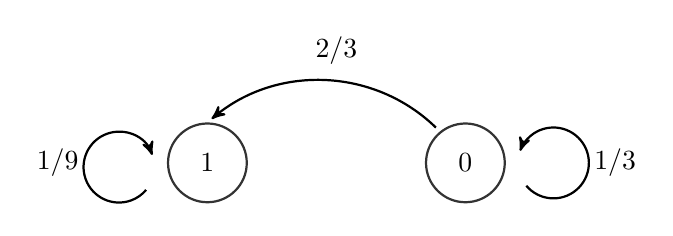
\begin{tikzpicture}[
rno/.style={circle, draw=black!80, fill=green!0,  thick, minimum size=10mm},
rnoin/.style={circle, draw=black!60,   thick, minimum size=10mm},
 % Define arrow style
    pil/.style={
           ->,
           thick,
           shorten <=2pt,
           shorten >=2pt,}
]
%Nodes
\draw[thick, <-] (-.7,.1) arc (20:320:.45);
\draw[thick, ->] (4.05,-.29) arc (220:520:.45);
%\draw[thick, ->] (1.4,-3.9) arc (130:430:.45);
\node[rno] (main1) {1};
\node (branch11) [left= of main1] {1/9};
\node (dum1) [right=of main1] {};
\node[rno] (main0) [right= of dum1] {0}
edge[pil, bend right=42] (main1.north);
\node (branch01) [above=of dum1] {2/3};
\node (branch00) [right= of main0] {1/3};
%\node (branch22) [below= of main2] {7/24};
\end{tikzpicture}
\caption{A three-state chain without efficient coupling.} \label{F1}
\end{figure}
\end{comment}

%
\section{At a threshold of 9.3 cm, the ``switch" between aerated and inundated can be modeled by a Dichotomous Markov process}
A known 2-state, continuous-time Markov chain (called a Dichotomous Markov chain, DMC) can be used to describe phenomenon when the permanence time of being in either state is exponentially distributed. In this case, our states are aerated (water table below 9.3 cm) and inundated (water table above 9.3 cm). If permanence times can be modeled by an exponential distribution, then we can use this well-known DMC model.  

Figure \ref{9.3_35bars} shows that the permanence time for aerated events (top) and inundated events (bottom) can be well-modeled by an exponential distribution. Here, permanence time is defined by the number of days water table spends either above or below the threshold value. 

Figure \ref{hists_thres} shows that at lower threshold values (0 and 5), permanence time is not as well-explained by an exponential distribution. 

%FIG ------------------------
%9.3_35bars
\begin{figure}[!htb]
\centering
\includegraphics[width=.45\textwidth]{permanence_times93_3bars}
\includegraphics[width=.45\textwidth]{permanence_times93_5bars}
\caption{Limited events makes distribution-fitting less reliable, though histograms line up relatively well to an exponential distribution. The left shows histogram events broken into 3 bars, while the right shows 5 bars. As resolution increases, gaps in the histogram appear due to the low count (17 events, e.g. 17 permanence times available) of events in the sample.  }\label{9.3_35bars}
\end{figure}

%FIG ------------------------
%hists_thres
\begin{figure}[!htb]
\centering
\includegraphics[width=\textwidth]{permanence_times_5bars}
\caption{Behavior at a threhold of 9.3 is decently explained by an exponential fit. Lower thresholds do not adhere to such a distribution well. Higher thresholds can be fitted with an exponential distribution as well, though, we need to consider other variables in defining the "best" threshold" value to use.  }\label{hists_thres}
\end{figure}

\section{The relationship between water table and expected methane emissions (based on soil temperature) changes depending on whether peat is aerated or saturated}
If expected methane emissions can't be further explained by these two states (aerated or inundated), then a model that switches between the two states will not be useful. Therefore, we need to show that there is a difference in methane emissions that can be explained by the state the system is in. 

\textbf{Hypothesis:}
When peat is aerated (as defined by a threshold of 9.3 cm), then higher water table will result in lower methane emissions than expected at that soil temperature. If peat is inundated, then higher water table (e.g. higher column of standing water since peat is already saturated) will result in higher methane emissions than expected at that soil temperature. 

Figure 3 demonstrates that hydrology does play a role in methane emissions. There is a significant positive relationship between water table depth and methane deviations (left). Further, the right hand side of Figure 3 shows that the methane deviations are related to water table in two opposing ways depending on whether the system is aerated (top right) or inundated (bottom right). Figures 4 and 5 further show that the intensity of this relationship (e.g. the slope) depends on how strict the threshold definition is. 

Results from Figures 3, 4 and 5 motivate the following section.

%FIG 3
\begin{figure}[!htb]
\centering
\includegraphics[width=.8\textwidth]{A2l}
\includegraphics[width=.8\textwidth]{I2l}
\caption{The figures on the left show that there is slight positive relationship between water table and expected methane release. The figures on the right show that this relationship changes dramatically when we mask out either aerated or inundated events.  }
\end{figure}

%FIG 4
\begin{figure}[!htb]
\centering
\includegraphics[width=.8\textwidth]{A93l}
\caption{If aerated events are defined to be those such that water table is below 9.3 cm, then water table is negatively correlated with expected methane deviations. This is true too for lower threshold, like 5 cm, and in fact, the lower the threshold (and so the stricter the definition of an aerated event), the steeper the negative slope. At a threshold of 14; however, this relationship becomes positive.   }
\end{figure}

%FIG 5
\begin{figure}[!htb]
\centering
\includegraphics[width=.8\textwidth]{I93l}
\caption{For inundated events, there is a positive correlation between water table and methane deviations. The more strict this definition of inundation (e.g. the higher the threshold), the steeper the slope between water table and methane deviations becomes.    }
\end{figure}

\section{Water table vs. methane deviations as a quadratic function}
In previous sections, we often used a threshold of 9.3 cm. In general, threshold values above 9 result in permanence times that are explained relatively well by exponential distributions. This is partly why the threshold of 9.3 is used. However, perhaps the switch in water table-methane deviations behavior is better explained by a higher or lower threshold value. 

Results from Figures 3, 4 and 5 motivate us to fit our water table-methane deviations graph with a quadratic function; however, quadratic functions are symmetrical and Figures 4 and 5 indicate that this is likely not the case seeing as slope changes at different rates for different threshold values depending on whether or not the data we're fitting is aerated or inundated. This is best exemplified by the bottom two graphs in Figure 4 and in Figure 5. In Figure 4, the slope changes from negative for aerated events defined by a 9.3 cm threshold and \textit{positive} for aerated events as defined by a 14 cm threshold. In Figure 5 (inundated events), we never see a shift from a positive to negative slope despite use of the same threshold values. In other words, the rate of change of \textit{slope itself} is not the same for inundated and aerated events, so a were quadratic fitting will not capture this lack of symmetry. 

Naively, we fit a quadratic function while masking aerated/inundated events in Figure \ref{quad}. 
\begin{figure}[!htb]
\centering
\includegraphics[width=.45\textwidth]{Ap}
\includegraphics[width=.45\textwidth]{Ip}
\caption{We see functional minimum values ranging from a water table depths of 2.3 and 13.6. Thus, a threshold value of 9.3 cm is reasonable.}\label{quad}
\end{figure}











\end{document}